\section{Arquitectura de Persistencia, CDC y Plataforma Web}
\label{sec:arquitectura_datos}

Para superar las limitaciones inherentes a los archivos planos y permitir la interoperabilidad transaccional multiusuario, el proyecto evolucionó desde una base de datos local embebida hacia una arquitectura distribuida basada en \emph{Neon Serverless PostgreSQL} (compatible con versiones 17.5 y 18.x), alojada en la nube con conexión cifrada SSL obligatoria (\texttt{sslmode=require}).

\subsection{Esquema Físico Relacional y Modelado de Datos}

El modelo relacional está compuesto por 16 tablas organizadas en cuatro subsistemas lógicos:
\begin{enumerate}[label=\alph*)]
  \item \textbf{Catálogo Académico Institucional:} Tablas \texttt{docentes}, \texttt{materias} y \texttt{oferta\_}\allowbreak\texttt{academica\_}\allowbreak\texttt{semestral}. Modela la estructura curricular de la Carrera de Informática de la UMSA y gestiona la evolución temporal de asignaturas y paralelos mediante una estrategia de dimensión de cambio lento (SCD Tipo 2).
  \item \textbf{Tabla de Hechos Central:} La tabla \texttt{mensajes} almacena los 23.371 mensajes del corpus, desnormalizando atributos calculados de alto acceso (polaridad léxica, emoción dominante, banderas multimodales para OCR, stickers y GIFs, e índices numéricos de intensidad afectiva).
  \item \textbf{Matrices Analíticas de Alta Densidad:} Las tablas \texttt{tfidf\_mensajes} (122.971 registros ponderados), \texttt{ngrams\_frecuencias} (27.334 filas) y \texttt{metricas\_temporales} desacoplan el cálculo computacional intensivo de la capa de visualización.
  \item \textbf{Trazabilidad y Menciones Académicas:} La tabla \texttt{menciones\_docentes} vincula los mensajes con las entidades docentes identificadas mediante expresiones regulares compiladas (\texttt{alias\_regex}).
\end{enumerate}

\begin{table}[htbp]
  \centering
  \small
  \caption{Métricas Operativas Globales y Composición Multimodal del Corpus de la UMSA}
  \label{tab:kpis_corpus}
  \resizebox{\textwidth}{!}{
  \begin{tabular}{lrr}
    \toprule
    Métrica / Dimensión & Valor Observado & Observación Metodológica \\
    \midrule
    Total de mensajes persistidos          & 23.371 & Corpus histórico consolidado en Neon PostgreSQL \\
    Usuarios únicos remitentes             & 2.051  & Estudiantes, auxiliares y coordinadores \\
    Promedio de mensajes por usuario       & 11,4   & Distribución de cola larga con alta dispersión \\
    Total de elementos multimodales        & 4.919  & Imágenes, stickers y animaciones GIF \\
    Imágenes procesadas con OCR            & 1.782  & Capturas de comunicados y boletas de inscripción \\
    Stickers analizados                    & 2.180  & Clasificados por carga afectiva y emoji asociado \\
    Animaciones GIF documentadas           & 24     & Reacciones animadas catalogadas \\
    Reacciones interactivas de Telegram    & 2.575  & Emojis directos en globos de mensaje \\
    Modismos y jergas locales de la UMSA   & 538    & Catálogo léxico contextual paceño \\
    Términos procesados en TF-IDF          & 122.971 & Matriz dispersa de términos ponderados \\
    \bottomrule
  \end{tabular}
  }
  \vspace{4pt}
  \begin{minipage}{0.94\textwidth}
    \footnotesize
    \textit{Nota.} Datos extraídos en tiempo real desde las tablas operativas \texttt{mensajes}, \texttt{menciones\_docentes} y \texttt{tfidf\_mensajes} en Neon Serverless PostgreSQL (región AWS us-east-2 / sa-east-1).
  \end{minipage}
\end{table}


La Figura~\ref{fig:erd_neon_schema} presenta el diagrama entidad-relación (ERD) completo del modelo físico implementado en Neon PostgreSQL, detallando las relaciones de cardinalidad entre el núcleo transaccional, los catálogos y las vistas analíticas materializadas.

\begin{figure}[htbp]
  \centering
  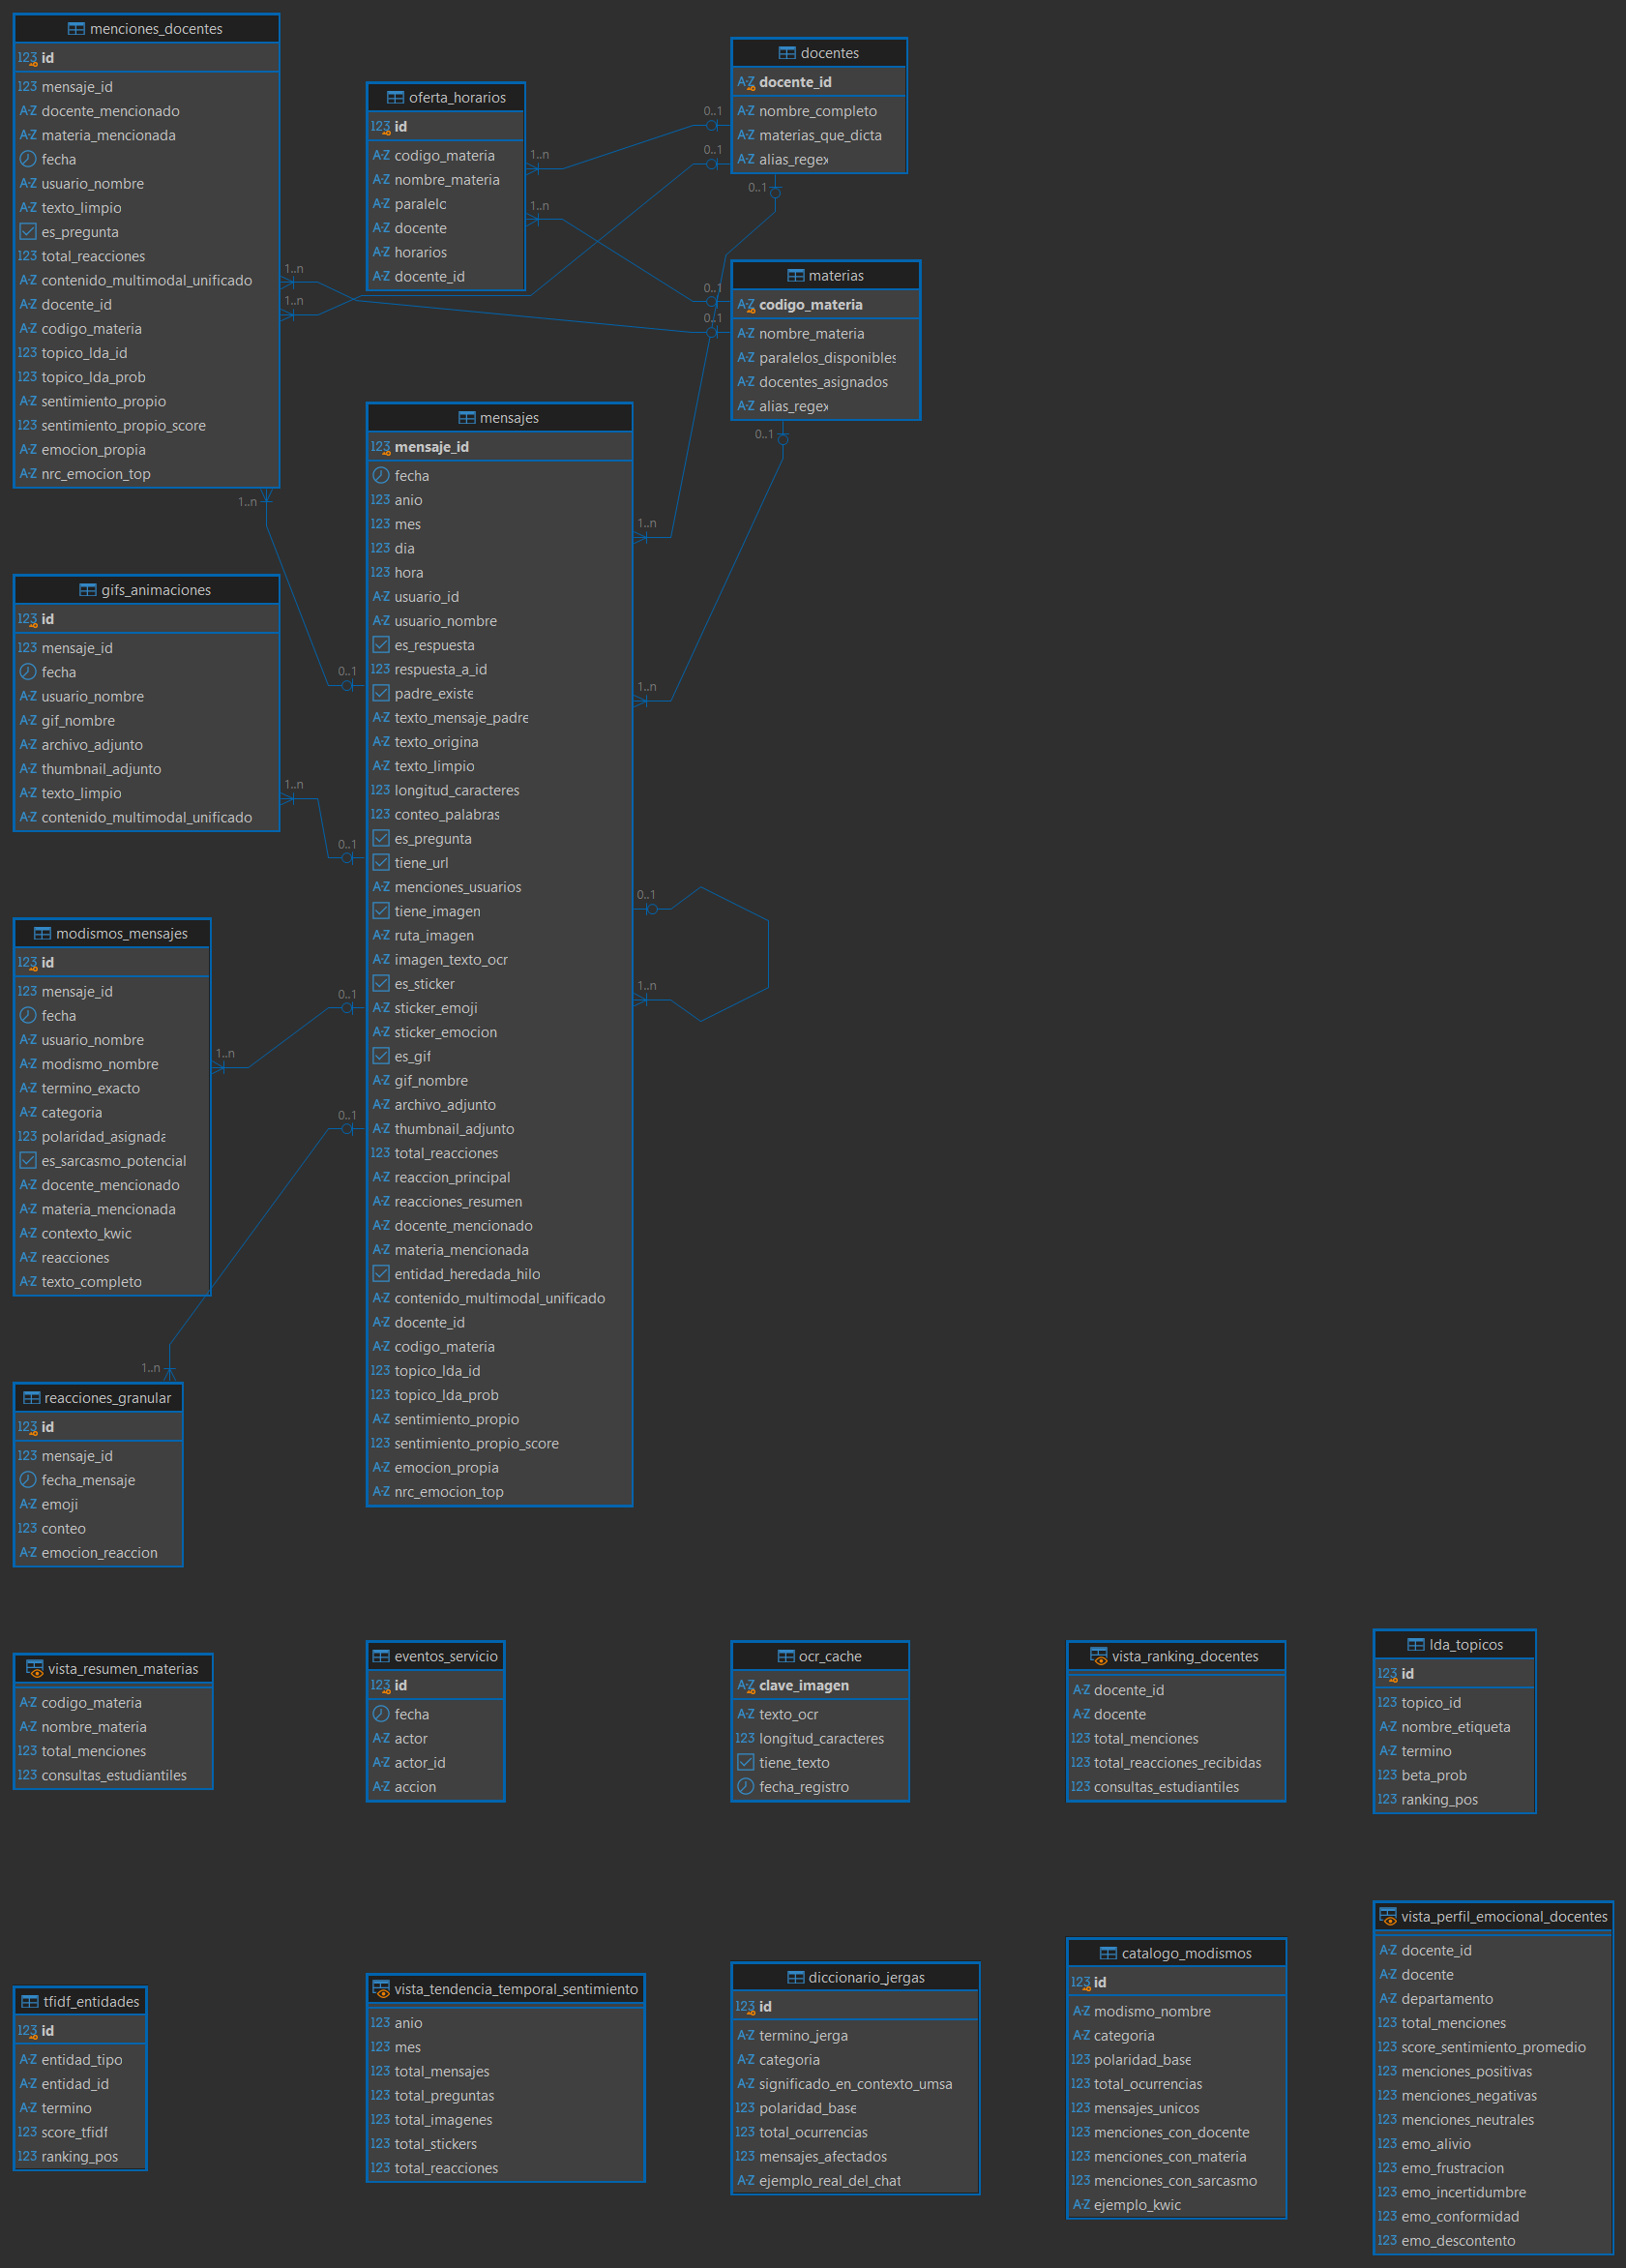
\includegraphics[width=0.88\textwidth]{figures/CAP17JNAC_db.png}
  \vspace{4pt}
  \caption{Diagrama Entidad-Relación (ERD) del esquema físico en Neon Serverless PostgreSQL (16 tablas y vistas analíticas).}
  \label{fig:erd_neon_schema}
\end{figure}

\subsection{Captura de Cambios de Datos en Tiempo Real (CDC)}

La trazabilidad del sistema se garantiza a nivel de motor de base de datos mediante la tabla \texttt{bitacora\_cambios} y una función disparadora genérica (\texttt{fn\_registrar\_bitacora\_cambio()}) escrita en PL/pgSQL (Listado~\ref{lst:cdc_trigger}). Ante cualquier operación de actualización (\texttt{UPDATE}) o eliminación (\texttt{DELETE}), el trigger intercepta los registros \texttt{OLD} y \texttt{NEW}, compara campo por campo utilizando funciones de introspección JSONB y genera un delta granular (\texttt{diff\_modificaciones}).

\begin{lstlisting}[language=SQL, caption={Funcion trigger PL/pgSQL para captura diferencial de cambios (CDC) en formato JSONB}, label={lst:cdc_trigger}]
CREATE OR REPLACE FUNCTION fn_registrar_bitacora_cambio()
RETURNS TRIGGER AS $$
DECLARE
    v_old_json JSONB := NULL;
    v_new_json JSONB := NULL;
    v_diff JSONB := '{}'::JSONB;
    v_key TEXT;
    v_pk_val TEXT := NULL;
BEGIN
    IF (TG_OP = 'UPDATE') THEN
        v_old_json := to_jsonb(OLD);
        v_new_json := to_jsonb(NEW);
        v_pk_val := COALESCE(v_new_json->>'message_id', v_new_json->>'id');

        -- Deteccion granular de atributos modificados
        FOR v_key IN SELECT jsonb_object_keys(v_new_json)
        LOOP
            IF v_new_json->v_key IS DISTINCT FROM v_old_json->v_key THEN
                v_diff := v_diff || jsonb_build_object(
                    v_key, jsonb_build_object('anterior', v_old_json->v_key, 'nuevo', v_new_json->v_key)
                );
            END IF;
        END LOOP;

        IF v_diff <> '{}'::JSONB THEN
            INSERT INTO bitacora_cambios (
                tabla_afectada, operacion, registro_id, datos_previos,
                datos_nuevos, diff_modificaciones, fecha_hora
            ) VALUES (
                TG_TABLE_NAME, TG_OP, v_pk_val, v_old_json, v_new_json, v_diff, clock_timestamp()
            );
        END IF;
        RETURN NEW;
    END IF;
    RETURN NULL;
END;
$$ LANGUAGE plpgsql SECURITY DEFINER;
\end{lstlisting}


En la interfaz de supervisión de SentiDataUMSA, este subsistema de gobernanza se descompone en tres pantallas operativas: la Figura~\ref{fig:ui_bitacora_general} exhibe la bitácora transaccional y el registro de eventos del sistema; la Figura~\ref{fig:ui_pipeline_linaje} muestra el linaje de pipelines registrado cronológicamente para cada una de las cinco fases de transformación; y la Figura~\ref{fig:ui_cdc_auditoria} presenta la consola de auditoría CDC en vivo, evidenciando las mutaciones capturadas por el disparador PL/pgSQL con el diff granular de modificaciones en los campos de expresiones regulares (\texttt{alias\_regex}).

\begin{figure}[htbp]
  \centering
  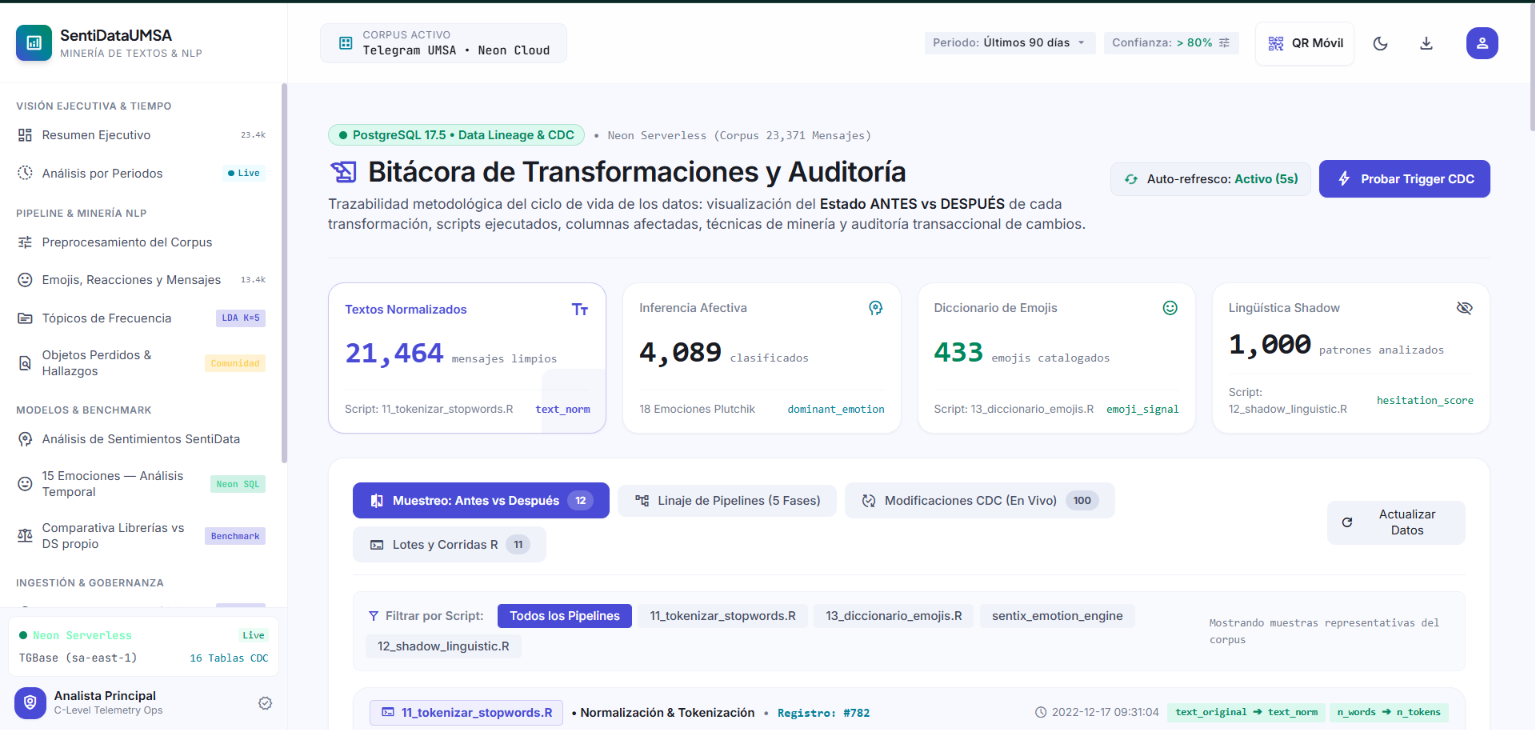
\includegraphics[width=0.92\textwidth]{figures/CAP26JNAC.png}
  \vspace{4pt}
  \caption{Bitácora transaccional y consola de supervisión de gobernanza de datos en SentiDataUMSA.}
  \label{fig:ui_bitacora_general}
\end{figure}

\begin{figure}[htbp]
  \centering
  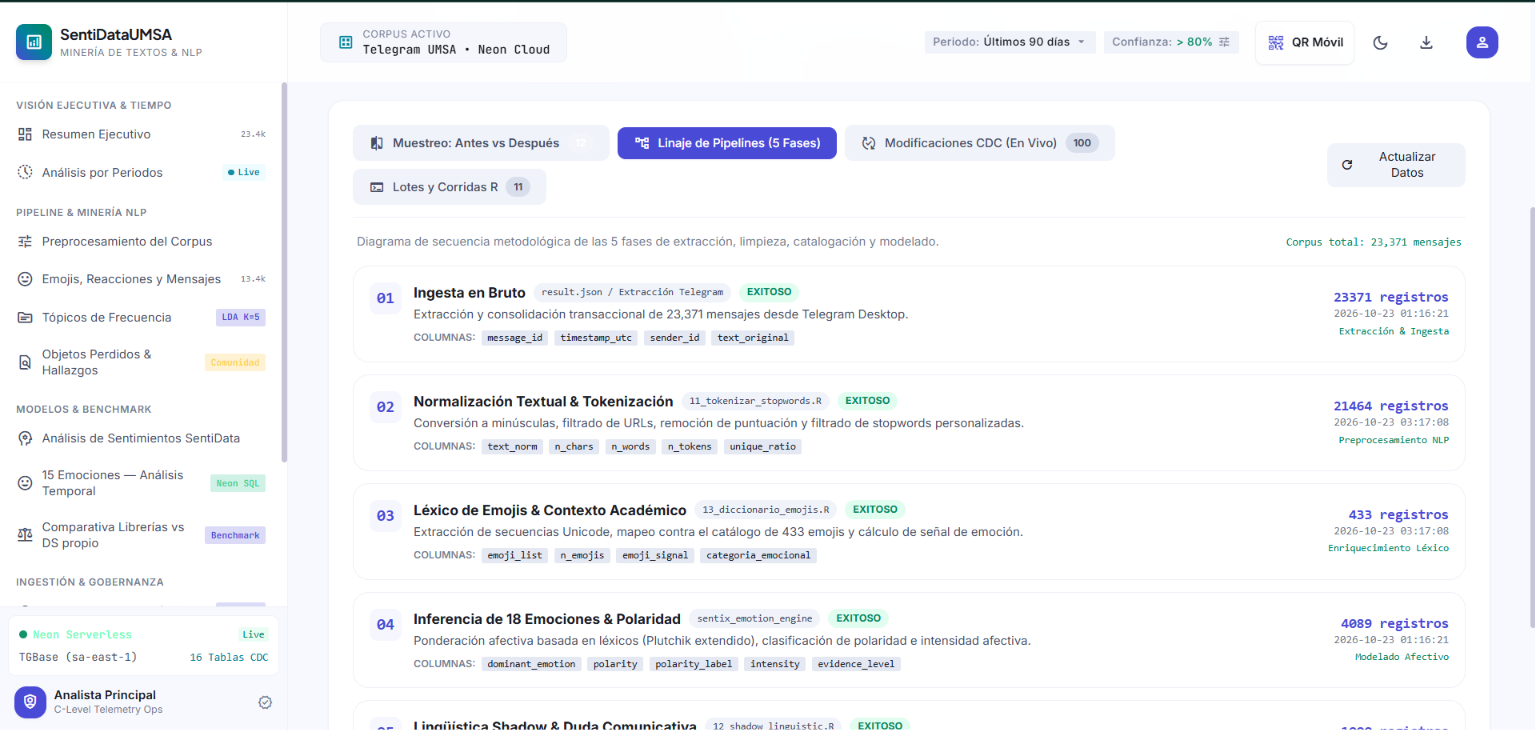
\includegraphics[width=0.92\textwidth]{figures/CAP27JNAC.png}
  \vspace{4pt}
  \caption{Linaje de ejecución de las cinco fases del pipeline de minería y transformación de datos en la bitácora.}
  \label{fig:ui_pipeline_linaje}
\end{figure}

\begin{figure}[htbp]
  \centering
  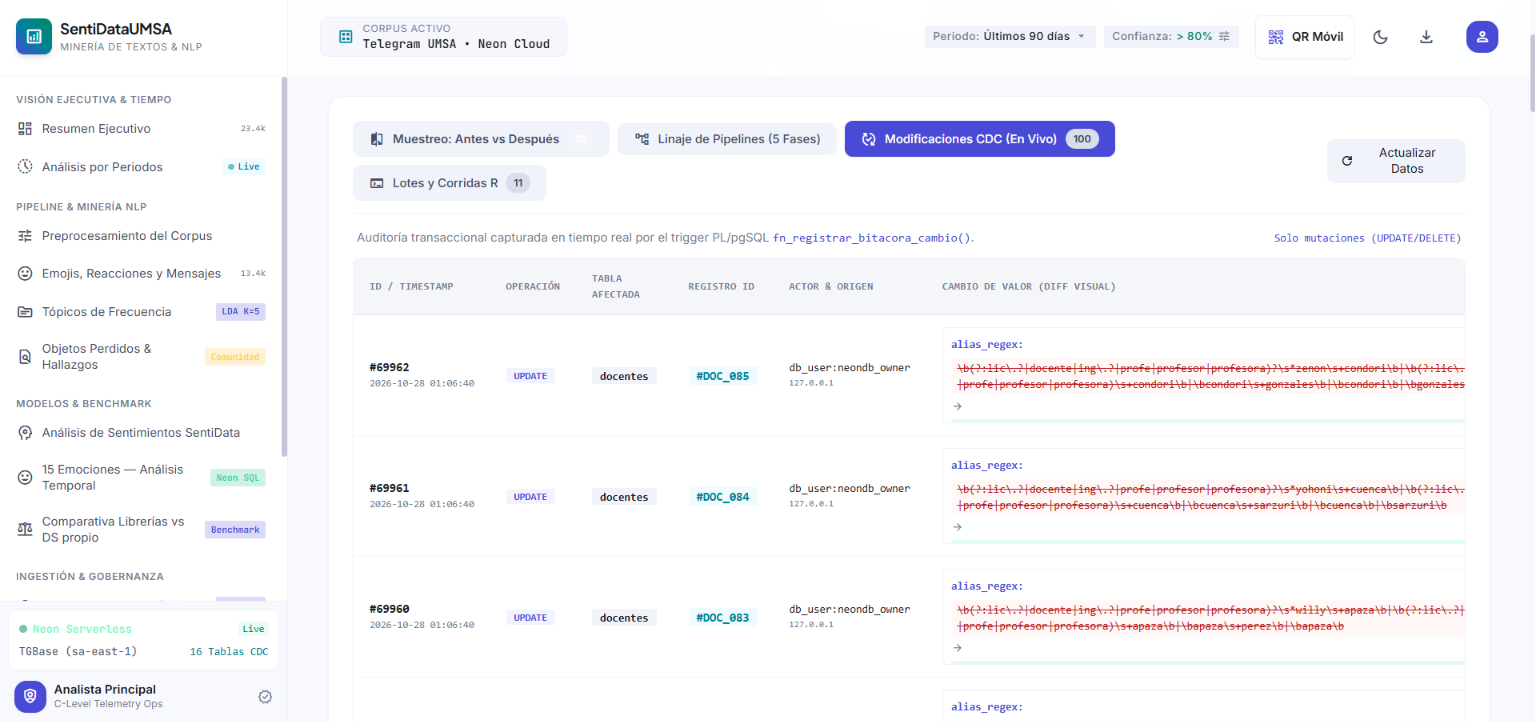
\includegraphics[width=0.92\textwidth]{figures/CAP28JNAC.png}
  \vspace{4pt}
  \caption{Auditoría transaccional en tiempo real con Change Data Capture (CDC) y diferenciación de mutaciones del trigger PL/pgSQL.}
  \label{fig:ui_cdc_auditoria}
\end{figure}

\subsubsection{Optimización y Prevención de Amplificación de Escritura}
Durante la fase experimental, la inserción masiva de 12.581 tokens y registros lingüísticos generó un fenómeno de amplificación de escritura (\emph{write amplification}), saturando la bitácora con más de 12.000 eventos atómicos. Como solución ingenieril documentada en el script \texttt{optimize\_bitacora.py}, se desactivaron los triggers de fila sobre tablas analíticas transitorias (\texttt{tokens\_frecuencia} y \texttt{shadow\_linguistics}), canalizando la trazabilidad de lotes hacia \texttt{bitacora\_procesos\_mineria} (Figura~\ref{fig:ui_lotes_mineria}).

\begin{figure}[htbp]
  \centering
  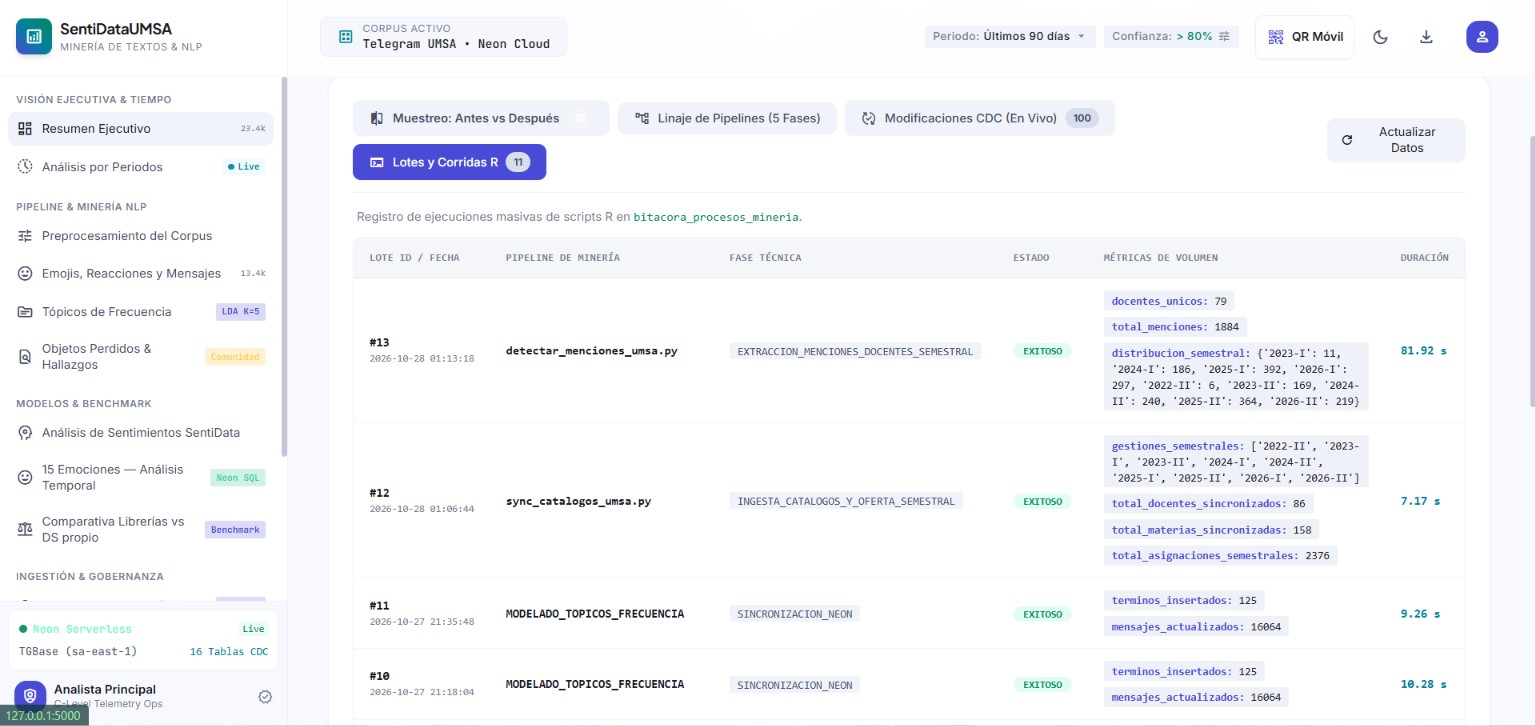
\includegraphics[width=0.92\textwidth]{figures/CAP29JNAC.png}
  \vspace{4pt}
  \caption{Gestión y auditoría de lotes de procesos de minería de datos y sincronización analítica.}
  \label{fig:ui_lotes_mineria}
\end{figure}

\subsection{Plataforma Web y Analítica Visual en Tiempo Real}

El consumo de datos y la interacción del usuario se centralizan en una aplicación web modular desarrollada en Python mediante el microframework Flask \citep{grinberg2018flask}, organizada bajo el patrón \emph{Application Factory} con dos Blueprints:
\begin{itemize}
  \item \textbf{Blueprint Web (\texttt{app/routes/web}):} Renderizado del lado del servidor (SSR) mediante plantillas Jinja2, diseño responsive basado en tokens de Material Design 3, modo oscuro nativo anti-FOUC y visualizadores especializados.
  \item \textbf{Blueprint API REST v1 (\texttt{app/routes/api\_v1}):} Endpoints de telemetría y el controlador de ingesta (\texttt{/api/v1/ingest/upload}).
\end{itemize}

La Figura~\ref{fig:ui_dashboard_ejecutivo} exhibe la pantalla de inicio del tablero de control (Dashboard C-Level), donde convergen los indicadores ejecutivos de telemetría, el gráfico interactivo donut de composición multimodal y el ranking superior de docentes con mayores menciones estudiantiles.

\begin{figure}[htbp]
  \centering
  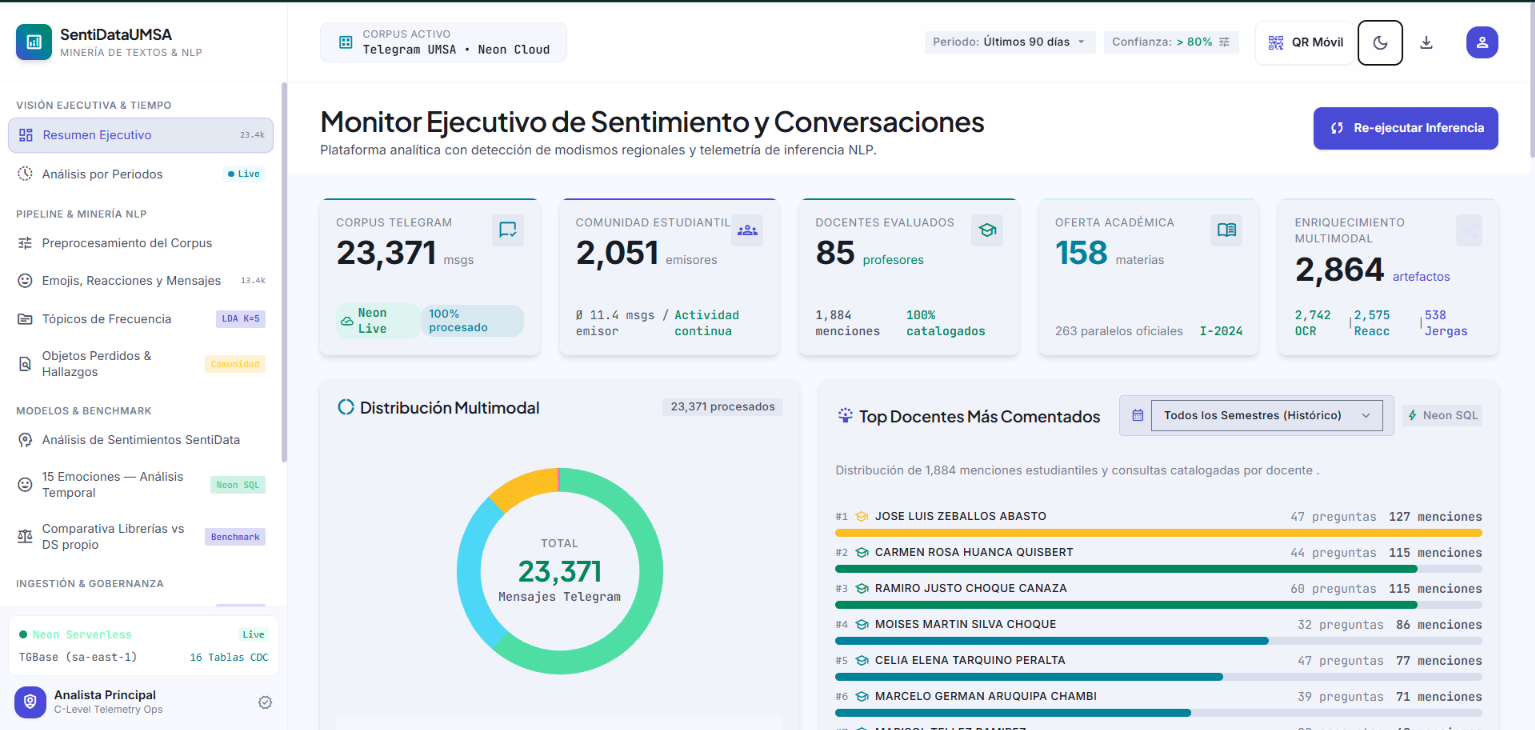
\includegraphics[width=0.92\textwidth]{figures/CAP1JNAC.png}
  \vspace{4pt}
  \caption{Panel de control ejecutivo (Dashboard C-Level) de la plataforma SentiDataUMSA.}
  \label{fig:ui_dashboard_ejecutivo}
\end{figure}

\subsubsection{Aislamiento In-Memory para Ingesta Multimodal}
Para proteger la integridad del corpus oficial de la UMSA, la subida de nuevos paquetes de chat (archivos JSON o archivos comprimidos ZIP de Telegram Desktop con imágenes y stickers) opera bajo un esquema de \emph{aislamiento de escritura cero} (\emph{zero-write isolation}). Tal como se aprecia en el Listado~\ref{lst:ingest_memory}, el motor en Python parsea, normaliza y puntúa las emociones íntegramente en memoria RAM, realizando únicamente consultas de solo lectura (\texttt{SELECT}) a Neon PostgreSQL para contrastar el nuevo chat contra el promedio histórico.

\begin{lstlisting}[language=Python, caption={Ingesta en memoria con aislamiento de transacciones de escritura (\texttt{ingest.py})}, label={lst:ingest_memory}]
@api_v1_bp.route("/ingest/upload", methods=["POST"])
def ingest_upload_view():
    """
    Procesa lotes de Telegram (JSON o ZIP) 100% en memoria en Python.
    Compara las metricas resultantes contra el baseline de Neon (Read-Only).
    """
    archivos = request.files.getlist("files")
    if not archivos:
        return jsonify({"error": "No se recibieron archivos"}), 400

    # 1. Parseo y extraccion en memoria sin mutacion de base de datos
    df_mensajes = parsear_paquete_telegram(archivos)
    
    # 2. Preprocesamiento y scoring lexico
    df_limpio = preprocess_chat(df_mensajes)
    scores_df = score_emotions(df_limpio)
    
    # 3. Consulta de solo lectura (SELECT) contra Neon PostgreSQL
    baseline = consultar_baseline_corpus_neon()
    timeline = calcular_timeline_chat(df_limpio)

    return jsonify({
        "status": "success",
        "total_mensajes": len(df_mensajes),
        "timeline": timeline,
        "comparativa_neon": {"chat": scores_df, "baseline": baseline}
    }), 200
\end{lstlisting}


La Figura~\ref{fig:ui_ingesta_inmemory} muestra la interfaz de usuario implementada para este mecanismo, donde el usuario puede arrastrar paquetes exportados de Telegram Desktop mientras el sistema garantiza que la base de datos Neon permanezca intacta en modo de solo lectura.

\begin{figure}[htbp]
  \centering
  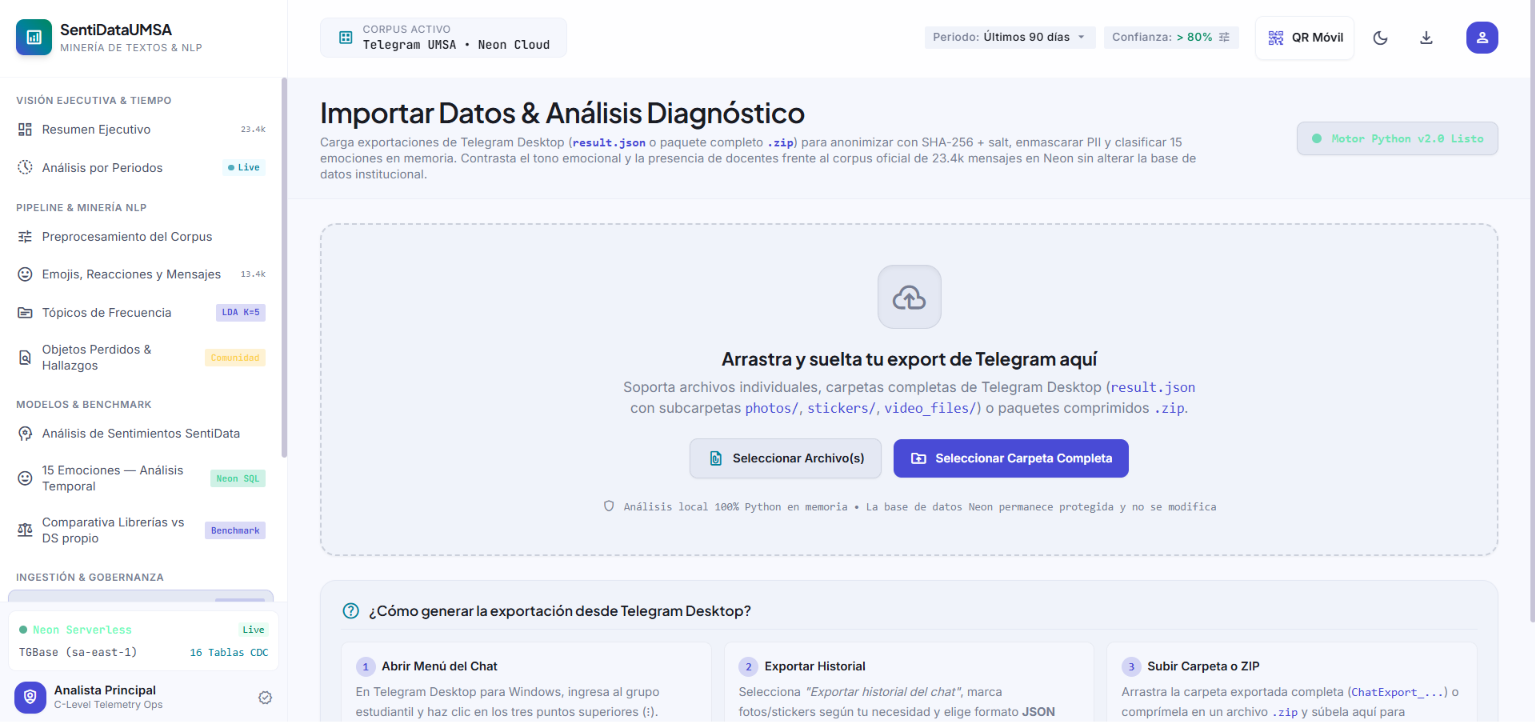
\includegraphics[width=0.92\textwidth]{figures/CAP25JNAC.png}
  \vspace{4pt}
  \caption{Módulo de ingesta y gobernanza de datos con aislamiento de memoria y protección transaccional de escritura cero.}
  \label{fig:ui_ingesta_inmemory}
\end{figure}

\subsubsection{Ingeniería de Motores Gráficos Especializados}
A diferencia de tableros convencionales que delegan la representación a bibliotecas genéricas rígidas, la plataforma incorpora dos motores visuales avanzados:
\begin{enumerate}
  \item \textbf{Motor Spline SVG Nativo (\texttt{timeline\_chart.js}):} Renderiza curvas continuas de Bézier sobre el DOM mediante elementos vectoriales \texttt{<path>}, soportando selector dinámico de granularidad (anual, semestral, mensual, 24 horas), crosshair magnético con interpolación de coordenadas y tooltips glassmórficos.
  \item \textbf{Flujo ETL en Sankey (\texttt{sankey\_engine.js}):} Emplea Apache ECharts para graficar la reducción de dimensionalidad y pérdida de volumen del dato desde su estado crudo hasta los tokens afectivos útiles.
\end{enumerate}
